% chktex-file 3 chktex-file 18 chktex-file 36 chktex-file 40
\section*{Exercise 2.6.}

Verify the calculations of $\phi_1$ and $\phi_2$ in Example 2.3.4. Also check that $X_3 = (2\cos \omega)X_2 - X_1$.

\textbf{Solution:}

We use Python's package sympy for the symbolic calculations of the following verifications of $\phi_1$ and $\phi_2$. In the example they say that $\phi_n$ is the solution for the following linear system
\[ \Gamma_n \phi_n = \gamma_n,\hspace{3em} \Gamma_n = [\gamma(i-j)]_{i,j = 1}^{n},\hspace{1em} \gamma_n = (\gamma(1),\ldots, \gamma(n))^T. \]

First, we import all the symbolic variables
\begin{minted}{python}
    import sympy as sp
    from sympy import cos, sin # cosine and sine functions
    from sympy.abc import t, h, A, B # variables t, h, A, B
    omega, sigma = sp.symbols("omega, sigma") # variables omega and sigma
\end{minted}

We define $X_t = A \cos (\omega t) + B \sin(\omega t)$ with the following line
\begin{minted}{python}
    X = lambda t: A*cos(omega*t) + B*sin(omega*t)
\end{minted}
Then, the autocovariance function $\gamma(h) = \sigma^2 \cos(\omega h)$
\begin{minted}{python}
    gamma = lambda h: sigma**2 * cos(omega*h)
\end{minted}
In the following two lines, we define $\Gamma_n$ and $\gamma_n$
\begin{minted}{python}
    Gamma_n = lambda n: sp.Matrix([[gamma(i-j) for i in range(1,n+1)] for j in range(1,n+1)])
    gamma_n = lambda n: sp.Matrix([gamma(i) for i in range(1,n+1)])
\end{minted}
We define $\phi_1$ and $\phi_2$, as follows
\begin{minted}{python}
    phi1 = sp.Matrix([cos(omega)])
    phi2 = sp.Matrix([2*cos(omega), -1])
\end{minted}

Finally, we verify $\Gamma_1 \phi_1 - \gamma_1 = [0]$ and $\Gamma_2 \phi_2 - \gamma_2 = [0,0]$ with the following lines
\begin{minted}{python}
    print(sp.trigsimp(Gamma_n(1)*phi1 - gamma_n(1)))
    print(sp.trigsimp(Gamma_n(2)*phi2 - gamma_n(2)))
\end{minted}
The function \mintinline{python}{sp.trigsimp} simplifies the trigonometric expression.

The output of the previous lines are: \mintinline{python}{Matrix([[0]])} and \mintinline{python}{Matrix([[0], [0]])} respectively.

\begin{figure}[H]
    \centering
    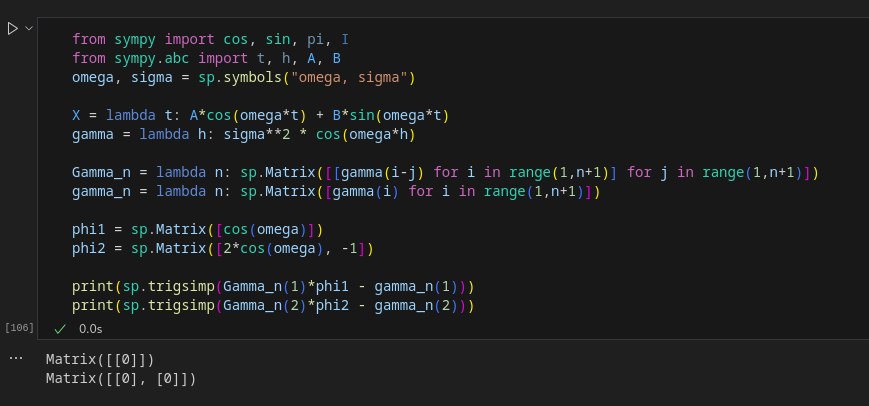
\includegraphics[width=0.95\textwidth]{../pictures/hw2ex2.6.1.png}
\end{figure}

Therefore, since the calculations made before are symbolic, $\phi_1$ and $\phi_2$ are the exact solutions to their respective linear systems. Finally, we verify that $X_3 - 2 \cos(w) X_2 + X_1 = 0$ with the following line
\begin{minted}{python}
    from sympy.simplify.fu import TR8
    expr = X(3) - 2*cos(omega)*X(2) + X(1)
    print(TR8(expr))
\end{minted}
What the function \mintinline{python}{TR8} does according to the \href{https://docs.sympy.org/latest/modules/simplify/fu.html}{documentation in this website} is to \textit{"expand products of sin-cos to sums"}. The output of the previous lines is \mintinline{python}{0} as we intended.

\begin{figure}[H]
    \centering
    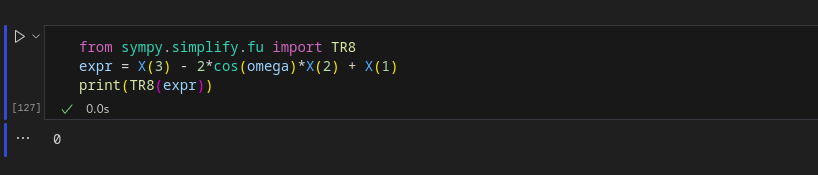
\includegraphics[width=0.95\textwidth]{../pictures/hw2ex2.6.2.png}
\end{figure}

This concludes the exercise.